\documentclass{article}
\usepackage{../../LaTeX/lambdatex} %disponibile all'indirizzo http://lambdamath.altervista.it/esercizi/lambdatex.sty
\usepackage{tasks}
\usepackage{exsheets}
\newcommand{\se}{\text{ se }}
\renewcommand{\phi}{\varphi}
\everymath{\displaystyle}


\title{Università degli Studi di Trento - Dipartimento di Matematica\\
CdL in Matematica – a.a. 2022–2023\\ Note esercitazione}
\author{Esercitatore: Simone Verzellesi\thanks{Trascrizione a cura di Davide Borra}}
\date{12 Dicembre 2022}
\begin{document}
\maketitle
\lhead{Note esercitazione}
\chead{Università degli Studi di Trento - Dipartimento di Matematica\\
CdL in Matematica – a.a. 2022–2023}
\rhead{12/12/2022}
\setlength{\headheight}{30pt}
% \begin{question}
%     pippo
%\end{question}
\begin{enumerate}[label=\textbf{Esercizio 12.\arabic*.},itemindent=*]
%%%%%%%%%%%%%%%%%%%%%%%%%%%%%%%%%%%%%%%%%%%%%%%%%%%%%
\item Siano $f(s)=\frac{e^{-|s|}-1}{s(s+1)}$ e $F(x)=\int_0^xf(s)ds$
\begin{tasks}
    \task Studiare $f(s)$
    \task Determinare $\dom F$
    \task Determinare $G_F$
\end{tasks}
\item[\textit{\large Soluzione~}]~
\begin{enumerate}
    \item Studiare $f(s)$
    \[f(s) = \begin{cases} \frac{e^{ - s} - 1}{s(s + 1)} &\se s > 0\\ \frac{e^{s} - 1}{s(s + 1)} &\se s < 0 \land s\neq - 1\end{cases} \]
    \begin{itemize}
        \item $\dom f=\R\setminus\{0,1\}$
        \item Segno di $f$:
        \[e^{-|s|}-1\leq 0~~\forall s\in \R\]
        \[s(s+1)>0~~\Harr~~s<-1\lor s>0.\]
        Quindi
        \[f(s)>0 \se -1<s<0\]
        \[f(s)<0 \se s <- 1 \lor s > 0\]
        \begin{figure}[h]
            \centering
            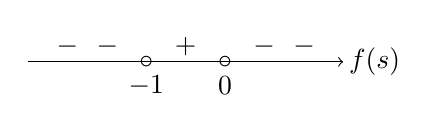
\begin{tikzpicture}
                \draw[->](-2.5,0)--(1.5,0);
                \node at(-1,0){$\circ$};
                \node at(-1,-0.3){$-1$};
                \node at(-0,0){$\circ$};
                \node at(0,-0.3){$0$};
                \node at(-1.75, 0.2){$- ~ ~-$};
                \node at(0.75, 0.2){$- ~ ~-$};
                \node at(-0.5, 0.2){$+$};
                \node at(1.9, 0){$f(s)$};
            \end{tikzpicture}
        \end{figure}
        \item Limiti
        \[\lim_{s\to-\infty}f(s)=0^-\]
        \[\lim_{s\to +\infty}f(s)=0^+\]
        \[\lim_{s\to1^-}f(s)=\left[ \frac{1-\frac{1}{e}}{0^-} \right]=-\infty\]
        \[\lim_{s\to1^+}f(s)=\left[ \frac{1-\frac{1}{e}}{0^+} \right]=+\infty\]
        \[\lim_{s\to0^-}f(s)=\lim_{s\to 0}\frac{e^s-1}{s(s+1)}\stackrel{LN}{=}1\]
        \[\lim_{s\to0^+}f(s)=\lim_{s\to 0}\frac{e^{-s}-1}{s(s+1)}\stackrel{LN}{=}-1\]
        \item Derivata di $f$
        \[f'(s)=\begin{cases}
            \frac{-e^{-s}(s^2+3s+1)+(2s+1)}{s^2(s+1)^2}&\se s>0\\
            \frac{e^{s}(s^2-s-1)+(2s+1)}{s^2(s+1)^2}&\se s<0 \land s \neq - 1\\
        \end{cases}\]
        \begin{itemize}
            \item se $s>0$
            \[f'(s) >0~~\Harr~~-e^{-s}(s^2+3s+1)+(2s+1)>0~~\Harr~~\frac{s^2+3s+1}{2s+1}<e^s\]
            Ora basta osservare ceh $e^s>s+1>\frac{s^2+3s+1}{2s+1}$.
            \item se $s<0 \land s\neq -1$ studiamo separatamente i due casi
            \begin{itemize}
                \item $-1<s<0$
                \[f'(s)<0~~\Harr~~e^s(s^2-s-1)+(2s+1)<0\]
                Poiché $e^s<1$, abbiamo che   \[e^s(s^2-s-1)<(s^2-s-1).\]Risulta quindi \[e^s(s^2-s-1)+(2s+1)<\underbrace{(s^2-s-1)+(2s+1)}_{s(s +1)}\]
                che è sempre negativo in $]0,1[$.
                \item $s<-1$
                \[f'(s)<0~~\Harr~~e^{s}(s^2-s-1)+(2s+1)<0~~\Harr~~-\frac{s^2-s-1}{2s+1}<e^{-s}\]
            Ora basta osservare che 
                \[e^{ - s} >- s + 1 > - \frac{s^2 - s - 1}{2s + 1}.\]
            \end{itemize}
        \end{itemize}
    \end{itemize}

    \begin{figure}[ht]
        \centering
        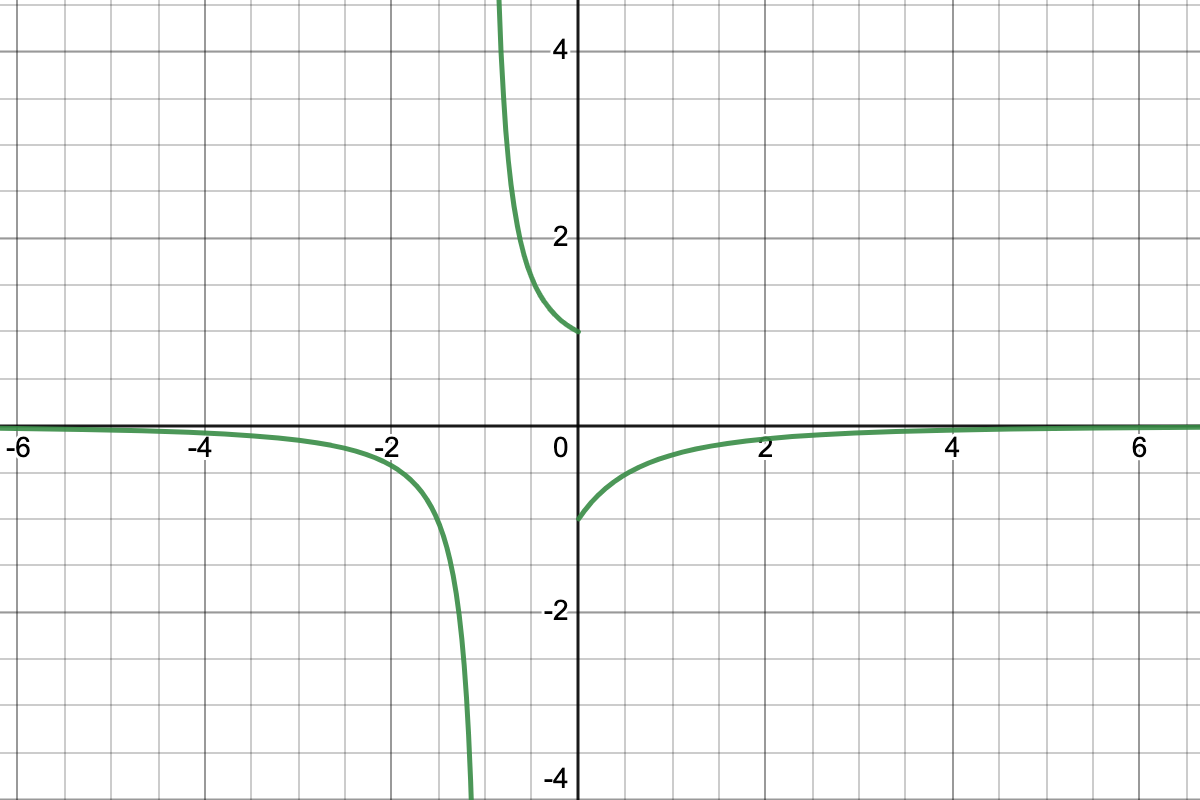
\includegraphics[width=0.6\textwidth]{src/disegno1.png}
        \caption{}
        \label{fig:1.1}
    \end{figure}

    \item Determinare $\dom F$.\\    
    Osserviamo che $0\in \dom F$ in quanto $F(0)=\int_0^0f(s)ds$
    \begin{itemize}
        \item se $x \in ]0,+\infty[$
        \[f(s)\underset{s\to0^+}{\longrightarrow}- 1\]
        e la funzione è continua in $]0,+\infty[$, per cui $f\in \mathcal{R}([0,\omega]), \forall \omega >0$, e quindi $]0,+\infty[\subset \dom F$.
        \item se $x\in]-1,0[$\\
        $f(s)$ è continua in $]-1,0[$ e $f(s)\underset{s\to0^-}{\longrightarrow}1$, per cui $f\in \mathcal{R}([a,0])~\forall a\in ~]-1,0[$.
        Dobbiamo controllare se l'integrale converge in $-1$
        \[\int_0^{-1}f(s)ds=\int_0^{-1}\frac{e^s-1}{s(s+1)}ds\]
        per $s\to-1^+$ si ha 
        \[\frac{e^s-1}{s(s+1)}\sim \frac{\frac{1}{e}-1}{-1(s+1)}=\left( 1-\frac{1}{e} \right)\left( \frac{1}{s+1} \right)\]
        quindi l'integrale diverge negativamente per il criterio del confronto asintotico, da cui
        \[]-\infty,-1]\nsubseteq\dom F\]
    \end{itemize}
    Abbiamo quindi che $\dom F=]-1;+\infty[$.
    \item Determinare $G_F$.\\
    Per definizione di funzione integrale sappiamo che $F(0)=0$, inoltre per il teorema fondamentale del calcolo
    \[F'(x)=f(x)\begin{cases}
        >0&\se -1<x<0\\
        <0&\se x>0
    \end{cases}\]
    \[F''(x)=f'(x)\begin{cases}
        <0&\se -1<x<0\\
        >0&\se x>0
    \end{cases}\]
    Per il corollario di Lagrange
    \[F'_-(0)=\lim_{x\to0^-}f(x)=1\neq -1=\lim_{x\to0^+}f(x)=F'_+(0)\]
    per cui in $x=0$ il grafico della funzione $F$ presenta un punto angoloso.
    Siamo quindi in grado di determinare il grafico di $F$ (Figura \ref{fig:1.2}):
    \begin{figure}[ht]
        \centering
        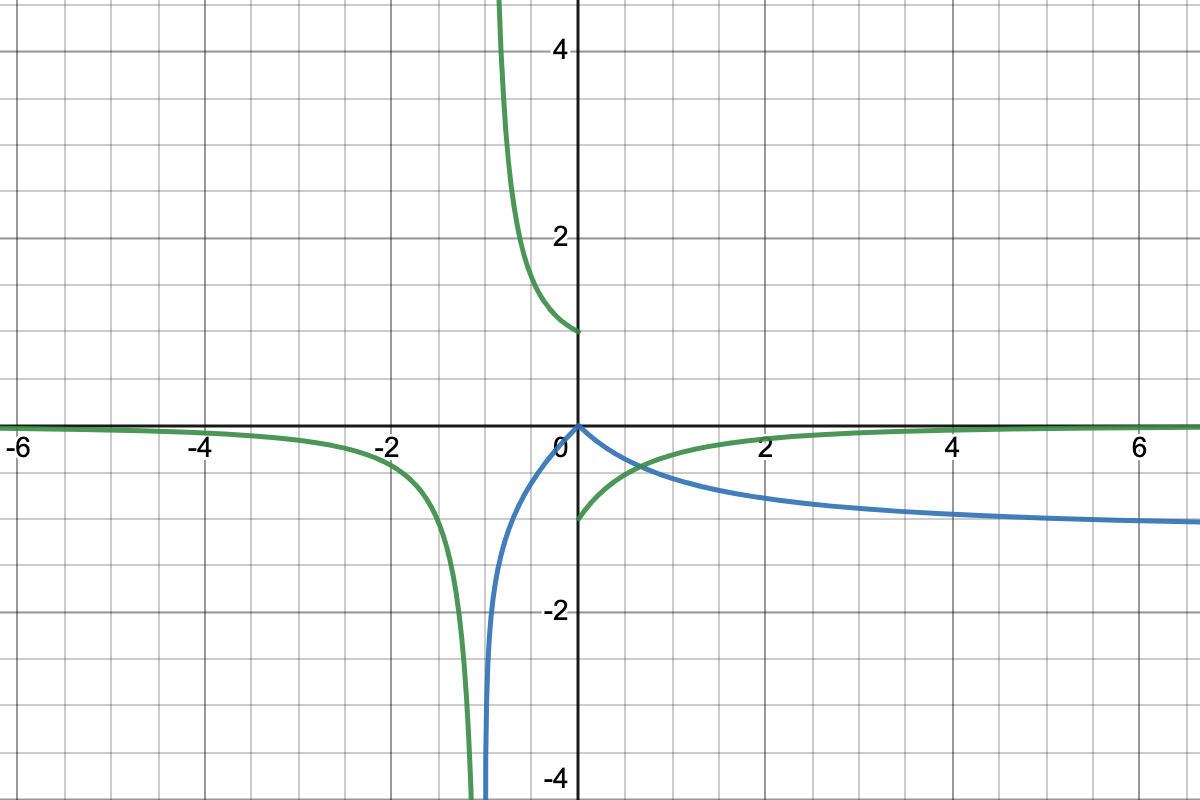
\includegraphics[width=0.6\textwidth]{src/disegno2.png}
        \caption{}
        \label{fig:1.2}
    \end{figure}
\end{enumerate}

%%%%%%%%%%%%%%%%%%%%%%%%%%%%%%%%%%%%%%%%%%%%%%%%%%%%%
Ricordiamo la definizione di convessità
\begin{shaded}
    \begin{definition}[Convessità]
        Sia $f:[a,b]\to\R$, $f$ si dice convessa se e solo se
        \[\forall x_1,x_2\in [a,b]:x_1 < x_2,\qquad f(x)\leq f(x_1)+\frac{f(x_2)-f(x_1)}{x_2-x_1}(x - x_1)\qquad \forall x\in[x_1,x_2] \]
    \end{definition}
\end{shaded}
\item Dimostrare che una funzione $f:[a,b]\to\R$ è convessa se e solo se vale la seguente disuguaglianza
\[f(\lambda x_1+(1-\lambda)x_2)\leq \lambda f(x_1)+(1-\lambda)f(x_2)~~~\forall \lambda \in [0,1], \forall x_1,x_2\in [a,b].\]
\item[\textit{\large Soluzione~}]~
\begin{proof}~
    \begin{itemize}
        \item \say{$\Rightarrow$}\\
        Prendo $x \in [x_1,x_2]$, allora posso scrivere $x=\lambda x_1+(1-\lambda)x_2$, con $\lambda\in[0,1]$
        \[\begin{aligned}f(x)&=f(\lambda x_1+(1-\lambda)x_2)\leq f(x_1) +\frac{f(x_2)-f(x_1)}{x_2-x_1}(\lambda x_1 +(1-\lambda )x_2-x_1) =\\
        &=f(x_1) +\frac{f(x_2)-f(x_1)}{\cancel{x_2-x_1}}(1-\lambda)\cancel{(x_2-x_1)} = f(x_1) + \left( f(x_2) - f(x_1) \right)(1 -\lambda) =\\&= \lambda f(x_1)+(1-\lambda)f(x_2).\end{aligned}\]
        \item \say{$\Leftarrow$}\\Prendo $x \in [x_1,x_2]$, allora posso scrivere $x=\frac{x_2-x}{x_2-x_1}x_1+\frac{x-x_1}{x_2-x_1}x_2$. Pongo $\lambda:=\frac{x_2-x}{x_2-x_1}\in[0,1]$. Allora $1-\lambda=\frac{x-x_1}{x_2-x_1}\in [0,1]$
        \[f(x)\leq \lambda f(x_1)+(1-\lambda)f(x_2)=\frac{x_2-x}{x_2-x_1}f(x_1)+\frac{x-x_1}{x_2-x_1}f(x_2)\]
        \[\implies f(x)\leq f(x_1) + (\frac{x_2-x}{x_2-x_1}-1)f(x_1)+\frac{x-x_1}{x_2-x_1}f(x_2) = f(x_1) +\frac{f(x_2) - f(x_1)}{x_2 - x_1}(x - x_1).\]
    \end{itemize}
\end{proof}
\item Provare che $f(x)=x^2$ è strettamente convessa.
\item[\textit{\large Soluzione~}]~
\begin{proof} Dobbiamo provare che
    \[f(\lambda x_1+(1-\lambda)x_2)<\lambda f(x_1)+(1-\lambda)f(x_2)~~~~~\forall \lambda \in ]0,1[\quad \forall x_1,x_2\in \R, x_1\neq x_2. \]
    Osserviamo che 
    \[(\lambda x_1+(1-\lambda)x_2)^2<\lambda x_1^2+(1-\lambda)x^2_2~~\Harr\]
    \[x_1^2\lambda(\lambda-1)+x_2^2((1-\lambda)^2-(1-\lambda))+2\lambda(1-\lambda)x_1x_2<0~~\Harr\]
    \[\lambda(\lambda-1)[x_1^2+x_2^2-2x_1x_2]<0\]
    \[\lambda(\lambda-1)(x_1-x_2)^2 < 0\]
    che è verificato $\forall \lambda \in ]0,1[, \forall x_1,x_2\in \R, x\neq x_1$.
\end{proof}
\item Dimostrare che $\forall a,b\geq 0, \forall p\in\R, p\geq 1$ vale
\[(a+b)^p\leq 2^{p-1}(a^p+b^p).\]
\item[\textit{\large Soluzione~}]~
\begin{proof} 
    Per $p=1$ la proprietà è ovvia. Se $a=0$ o $b=0$ la disuguaglianza è soddisfatta. Siano $a,b>0$, $p>1$. Pongo $f(t)=t^p$, che è una funzione convessa su $[0,+\infty[$ poiché $f''(t)=p(p-1)t^{p-2}>0$ su $]0,+\infty[$.Scelgo inoltre $x_1=a$ e $x_2=b$. Nella definizione precedente dell'Esercizio 12.2, si ha 
    \[(\lambda a +(1-\lambda)b)^p\leq \lambda a^p+(1-\lambda)b^p\]
    Scegliendo $\lambda=\frac{1}{2}$ si ottiene
    \[\left( \frac{1}{2} \right)^p(a+b)^p\leq \left( \frac{1}{2} \right)(a^p+b^p).\]
    e quindi
    \[(a+b)^p\leq 2^{p-1}(a^p+b^p).\]
\end{proof}
\item Sia $f:\R\to\R$ derivabile, si dimostri che $f$ è convessa se e solo se $\forall y \in \R$ \[f(x)\geq f(y)+f'(y)(x-y),\qquad \forall x \in \R .\]
\item[\textit{\large Soluzione~}]~
\begin{proof}
    %Per quanto detto prima, 
    %\[\frac{f(\lambda x+(1-\lambda)y)-f(y)}{\lambda}\leq \frac{\lambda (f(x)-f(y))}{\lambda}~~~\forall \lambda \in [0,1]\]
    %Allora, facendo tendere $\lambda$ a $0$ il secondo membro tende a 
    %\[\frac{f(\lambda x+(1-\lambda)y)-f(y)}{\lambda}\underset{\lambda \to 0}\longrightarrow f'(y)(x-y)~~~\Harr\]
    %Pongo $z=\lambda x+(1-\lambda)y$
    %\[f(x)\geq f(z)+f'(z)(x-z)\]
    %\[f(y)\geq f(z)+f'(z)(y-z)\]
    Se $x=y$ non c'è nulla da provare. Siano $x,y\in \R, x\neq y$ e sia $\lambda\in ]0,1]$. Abbiamo 
    \[f(\lambda x +(1 -\lambda )y)\leq \lambda f(x) + (1 -\lambda)f(y).\]
    Risulta
    \[ {\color{red}- f(y)} + f(y +\lambda(x - y))\leq \lambda f(x) +(1 -\lambda)f(y){\color{red}\, -\, f(y)}~ ~ \Harr\]
    \[\frac{f(y +\lambda(x - y))- f(y)}{\lambda} \leq \frac{\cancel\lambda (f(x) - f(y))}{\cancel\lambda}~ ~ \Harr\]
    \[(x - y)\frac{f(y +\lambda(x - y))- f(y)}{\lambda(x - y)} \leq f(x) - f(y)\]
    Passando al limite per $\lambda\to 0^+$, dalla derivabilità di $f$ segue 
    \[(x - y)f'(y)\leq f(x) - f(y)\]
    ossia 
    \[f(x)\geq f(y) + f'(y)(x - y).\]
    Per l'arbitrarietà di $x,y\in \R$, la dimostrazione è conclusa.
\end{proof}
\item \underline{\textit{Disuguaglianza di Young.}} Siano $p, q\in ]1;+\infty[$ tali che $\frac{1}{p}+\frac{1}{q}=1$. Dimostrare che $\forall a,b\geq 0$ 
\[ab\leq \frac{a^p}{p}+\frac{b^q}{q}.\]
\item[\textit{\large Soluzione~}]~
\begin{proof}
    Il caso $a=0$ o $b=0$ è banale, mentre il caso $p,q=2$ segue dal quadrato di binomio. Siano allora $a,b>0$.Siano $f(t)=\log(t)$, e $t_1=a^p, t_2=b^q, \lambda =\frac{1}{p}, 1-\lambda=1-\frac{1}{p}=\frac{1}{q}$.
    Allora sfruttando il fatto che la funzione $f$ è concava possiamo scrivere
    \[\log\left( \frac{a^p}{p}+\frac{b^q}{q} \right)\geq \frac{1}{p}\log(a^p) +\frac{1}{q}\log(b^q)\]
    da cui
    \[\log\left( \frac{a^p}{p}+\frac{b^q}{q} \right)\geq \log(a)+\log(b)=\log(ab)\]
    ne segue che 
    \[\frac{a^p}{p}+\frac{b^q}{q}\geq ab.\]
\end{proof}
\item \underline{\textit{Disuguaglianza di Hölder.}} \\Siano $p, q\in ]1;+\infty[$ tali che $\frac{1}{p}+\frac{1}{q}=1$. Dimostrare che $\forall (a_1, \dots, a_n), (b_1,\dots, b_n)\in \R^n$ con $a_i, b_i\geq 0~\forall i$ vale che 
\[\sum_{i=1}^n a_ib_i\leq \left(\sum_{i=1}^na_i^p\right)^{\frac{1}{p}}\cdot\left(\sum_{i=1}^nb_i^q\right)^{\frac{1}{q}}\]
\item[\textit{\large Soluzione~}]~
\begin{proof}
   Se $a_i=0~\forall i$ oppure $b_i=0~\forall i$ la disuguaglianza è ovvia. Supponiamo che $a_i\neq 0$ per qualche $i$ e $b_i\neq 0$ per qualche $i$. Poniamo $x_i=\frac{a_i}{\left(\sum\limits_{i=1}^na_i^p\right)^{\frac{1}{p}}}$ e $y_i=\frac{b_i}{\left(\sum\limits_{i=1}^nb_i^q\right)^{\frac{1}{q}}}$, allora segue che $x_i,y_i\geq 0~\forall i$.
   \\Per la disuguaglianza di Young $\forall i=1, \dots, n$ si ha
   \[x_iy_i\leq \frac{1}{p}x_i^p+\frac{1}{q}y_i^q.\]
   Quindi 
   \[\sum\limits_{i=1}^nx_iy_i\leq\sum\limits_{i=1}^n\left( \frac{1}{p}x_i^p+\frac{1}{q}y_i^q\right)=\frac{1}{p}\frac{\sum\limits_{i=1}^na_i^p}{\sum\limits_{i=1}^na_i^p}+\frac{1}{q}\frac{\sum\limits_{i=1}^nb_i^q}{\sum\limits_{i=1}^nb_i^q}=1.\]
   Da
   \[\sum_{i = 1}^nx_iy_i =\sum_{i = 1}^n\frac{a_i}{(\sum_{j = 1}^n a_j^p)^{\frac{1}{p}}}\frac{b_i}{(\sum_{j = 1}^n b_j^q)^{\frac{1}{q}}}\leq 1\]
   segue allora
   \[\sum_{i=1}^n a_ib_i\leq \left(\sum_{i=1}^na_i^p\right)^{\frac{1}{p}} \cdot \left(\sum_{i=1}^nb_i^q\right)^{\frac{1}{q}}.\]
\end{proof}

\begin{corollary*}[\underline{Disuguaglianza di Cauchy-Schwarz}]
    Siano $(a_1, \dots, a_n), (b_1,\dots, b_n)\in \R^n$ con $a_i, b_i\geq 0~~\forall i$, allora  
    \[\sum_{i=1}^n a_ib_i\leq \left(\sum_{i=1}^na_i^2\right)^{\frac{1}{2}}\left(\sum_{i=1}^nb_i^2\right)^{\frac{1}{2}}.\]
\end{corollary*}

\item \underline{\textit{Disuguaglianza di Jensen.}} Sia $f:\R\to\R, f\in \mathcal{C}^1(\R)$ convessa. Sia $g\in \mathcal{R}([a,b])$, allora 
\[f\left( \fint_a^b g(x)\d x \right)\leq \fint _a^bf(g(x))dx\] 
dove
\[\fint_a^bg(t)dt:=\frac{1}{b-a}\int _a^bg(t)dt.\]

\item[\textit{\large Soluzione~}]~

\begin{proof}
   Usando la caratterizzazione della convessità presentata precedentemente, nel caso $f$ derivabile (Esercizio 12.5), $\forall x\in [a,b]$
   \[f(g(x))\geq f\left(\fint_a^bg(t)dt\right)+f'\left(\fint_a^bg(t)dt\right)\left( g(x)-\fint _a^bg(t)dt \right)\]
   %\[\fint_a^bf(g(x))\geq\fint _a^b\left[f\left(\fint_a^b(g(t)dt)\right)+f'\left(\fint_a^bg(t)dt\right)\left( g(t)-\fint _a^bg(t)dt \right)\right]dx=\]
   %\[=f\left(\fint_a^bg(t)dt\right)+f'\left( \fint_a^bg(t)dt \right)\fint _a^b\left( g(x)-\fint _a^bg(t)dt \right)dx=\]
   %\[=f\left(\fint_a^bg(t)dt\right)+f'\left( \fint_a^bg(t)dt \right)\left[ \fint_a^bg(x)dx-\fint_a^bg(t)dt \right]\]
   %\[\implies \fint _a^b(f\circ g)(x)dx\geq f(\fint _a^bg(t)dt)\]
   Sfruttando la monotonia dell'integrale, integrando su $[a,b]$, si ha
   \[\int_a^bf(g(x))\d x\geq (b - a)f\left( \fint_a^bg(t)\d t \right) + f'\left( \fint_a^bg(t)\d t \right) \left( \int_a^bg(x)\d x -  \int_a^bg(t)\d t\right), \]
   cioè 
   \[\int_a^bf(g(x))\d x\geq (b - a)f\left(\fint_a^bg(t)\d t\right).\]
   Dividendo entrambi i membri per $(b-a)$ si ottiene la tesi.
\end{proof}

\item \underline{\textit{Disuguaglianza di Young generalizzata.}} Siano $p_1, \dots, p_n \in ]1;+\infty[$ tali che $\frac{1}{p_1}+\dots+\frac{1}{p_n}=1$. Dimostrare che 
\[\prod_{i=1}^na_i\leq \sum_{i=1}^n\frac{a_i^p}{p_i}\qquad \forall (a_1, a_2, \dots, a_n)\in \R^n, a_i\geq 0~\forall i.\]

\item[\textit{\large Soluzione~}]~
    Definiamo due nuove funzioni: $f(t)=\log(t)$ su $]0,+\infty[$ e $g:[0,1]\to \R$ 
    \[g(t)=\begin{cases}
        a_1^{p_1} &\se t \in[x_0, x_1[\\
        a_2^{p_2} &\se t \in [x_1, x_2[\\
        \:\vdots\\
        a_n^{p_n} &\se t \in [x_{n-1}, x_n]\\
    \end{cases}\]
    dove $x_0=0<x_1<x_<\dots<x_{n-1}<x_n=1$ e $x_i-x_{i-1}=\frac{1}{p_i}$.\\
    Siccome il logaritmo è una funzione concava, la disuguaglianza di Jensen si scrive $\forall g\in \mathcal{R}([0,1])$ come 
    \[f\left( \int_0^1 g(x)\d x\right)\geq\int_0^1f(g(x))\d x.\]
    Risulta allora per la funzioni $f$ e $g$ definite sopra
    \[\log\left( \sum_{i=1}^n\frac{a_i^{p_i}}{p_i} \right)\geq \sum_{i=1}^{p_i}\frac{1}{p_i}\log(a_i^{p_i})=\sum_{i=1}^n\log(a_i)=\log{\prod_{i=1}^n}a_i\]
    Passando all'esponenziale si ha la tesi.
\begin{flushright}
    \qed
\end{flushright}
\end{enumerate}
\end{document}
